



\documentclass[12pt,a4paper]{book}



			% Packages Files
%----------------------------------%

	% Page Setttings
\usepackage[top = 1in, bottom = 1in, left = 1in, right = 1in]{geometry}

\parindent=0cm % to prevent the spacing in new paragraph or new line

\usepackage{fancyhdr} % needded for header and footer 

%-----------------------------------------------------------------%

\usepackage{amsmath} % needed for referencing thequation
\usepackage{amsfonts} % for maths symbols
\usepackage{graphicx}
\usepackage[export]{adjustbox}
\usepackage{caption}
\usepackage{refstyle} % to reference a captioned figure


% To make hyperlinks

\usepackage[
	colorlinks=true
	,breaklinks
	]{hyperref} % needed for creating hyperlinks in the document, the option colorlinks=true gets rid of the awful boxes, breaklinks breaks lonkg links (list of figures),
	
\usepackage{xcolor}
\definecolor{c1}{rgb}{0,0,1} % blue
\definecolor{c2}{rgb}{0,0.3,0.9} % light blue
\definecolor{c3}{rgb}{0.3,0,0.9} % red blue
\hypersetup{
    linkcolor={c1}, % internal links
    citecolor={c2}, % citations
    urlcolor={c3} % external links/urls
}

	% For Code Writing
	
\usepackage{listings}

\usepackage{color}

\definecolor{mygreen}{rgb}{0 0.6 0}

\lstset{
% Set automatic Line breaking, in case we have long lines don't
% fit inside the frame or the page.
breaklines = true,
commentstyle = \color{mygreen},
breakatwhitespace = true,% don't show white space character
%numbers = left, % put line number in the code
title = \lstname
}

% ------------- For Writing Equations inisde a table and centering them ------------

\usepackage{array}

% Vertical Alignment inside the cells of the table
\newcolumntype{M}[1]{>{\centering\arraybackslash}m{#1}}

% Horizontal Alignment inside the cells of the table
\newcolumntype{P}[1]{>{\centering\arraybackslash}p{#1}}


% needed for todos liste
\usepackage{todonotes} 


\usepackage{nomencl}



% Macros File

% Macros Example
\def\labelaxes{Remember to include some suitable labeling for the axes and the units used in measurements.}

% 2nd way for defnining macros: the new command
% 1st parameter: name of the new command
% 2nd paramter: how many inputs this command needs, in this case only 1
% 3rd parameter: what this new command named \tbi do

\newcommand{\tbi}[1]{\textbf{\textit{#1}}}

% Command for Picture without a label

\newcommand{\pic}[3]{\begin{figure}[h]
\centering
\includegraphics[width = 0.7\textwidth, frame]{#1}
\caption{#2}
\end{figure}}








\DeclareMathOperator*{\argmax}{argmax} % thin space, limits underneath in displays

\DeclareMathOperator*{\argmin}{argmin}

\title{Sparsity and CS}
\author{Ranim Tom}



\begin{document}

% downloaded template
%\input{content/title_page_1} 

\maketitle
\tableofcontents

% to make the todo list appear as a table of content
\listoftodos


\pagestyle{fancy}
\fancyhf{} % Clear header and footer
\rhead{\rightmark}
\lhead{Chapter \thechapter}
\rfoot{Page \thepage}

\chapter*{Abstract}

This report contains my studies of sparse signal processing

\chapter{Introduction}

\section{Preliminaries}

In this section:

\begin{itemize}
    \item Introduce what is compressed sensing for
    
    \item Sparsity concepts
    
    \item Maybe some general notation
    
    \item Application of Sparse Signal Processing
    
\end{itemize}

This is to be developed after the writing of this manuscript

\section{Mathematical Modeling}


Let $x$ be some signal to be restored. It may be in the time domain, frequency domain,$\cdots$.

The problem to be solved: restore the original signal $x$, by using the sparse representation of $x$, its vector $s$, which are related by \autoref{Eq:Intro:sparsifying_a_signal}

\begin{equation}
x_{N \times 1} \, = \, \Psi_{N \times N} \, \times \, s_{N \times 1}
\label{Eq:Intro:sparsifying_a_signal}
\end{equation}

$\begin{cases}
\Psi_{N \times N}: \text{is some universal basis matrix (like DFT,DCT,$\cdots$ depending on what application we have)} \\
s_{N \times 1}: \text{is a sparse vector, where the number of non-zero elements is } K \ll N
\end{cases}$\\


The compressed sensing problem is defined as taking subsamples of $x$, which are denoted as the measurements $y$, solve for the sparse vector $s$ then restore $x$ via \autoref{Eq:Intro:sparsifying_a_signal}. These sequence of steps are translated in \autoref{Eq:Compressed_Sensing:formulation_2}

\begin{equation}
	\begin{array}{rcl}
	y_{m \times 1} \, &=& \, C_{m \, \times \, N} \,\times \,  x_{N \times 1} \\ 
		 &=& \, C_{m \, \times \, N} \, \times \, \Psi_{N \times N} \, \times \, s_{N \times 1} \\
		 &=& \, \Theta \, \times \, s_{N \times 1}
	\end{array}
\label{Eq:Compressed_Sensing:formulation_2}
\end{equation}

The system of equation by \autoref{Eq:Compressed_Sensing:formulation_2} is known to be an \tbi{undetermined} system: $\rightarrow$ there are infinite number of $s$ vectors which satisfy equation \autoref{Eq:Compressed_Sensing:formulation_2}


\newpage
\subsection{Example}

In this section, we run some simulation to compare the $\ell_1 ~$ and $\ell_2 ~$.\\

The purpose of this example is to emphasize that $\ell_1 ~$ promote sparse solution whereas $\ell_2 ~$ doesn't.\\

We take a sparse vector of dimension 1000, and the measurement vector $y$ is of dimension 200, implemented using the command \verb|measu_vect = randn(dimension_measurements,1)|\\

The matrix $\Theta$ is a random matrix implemented using the command \verb|Theta = randn(dimension_measurements,dimension_sparse_vector)|.



\begin{figure}[h]
\centering
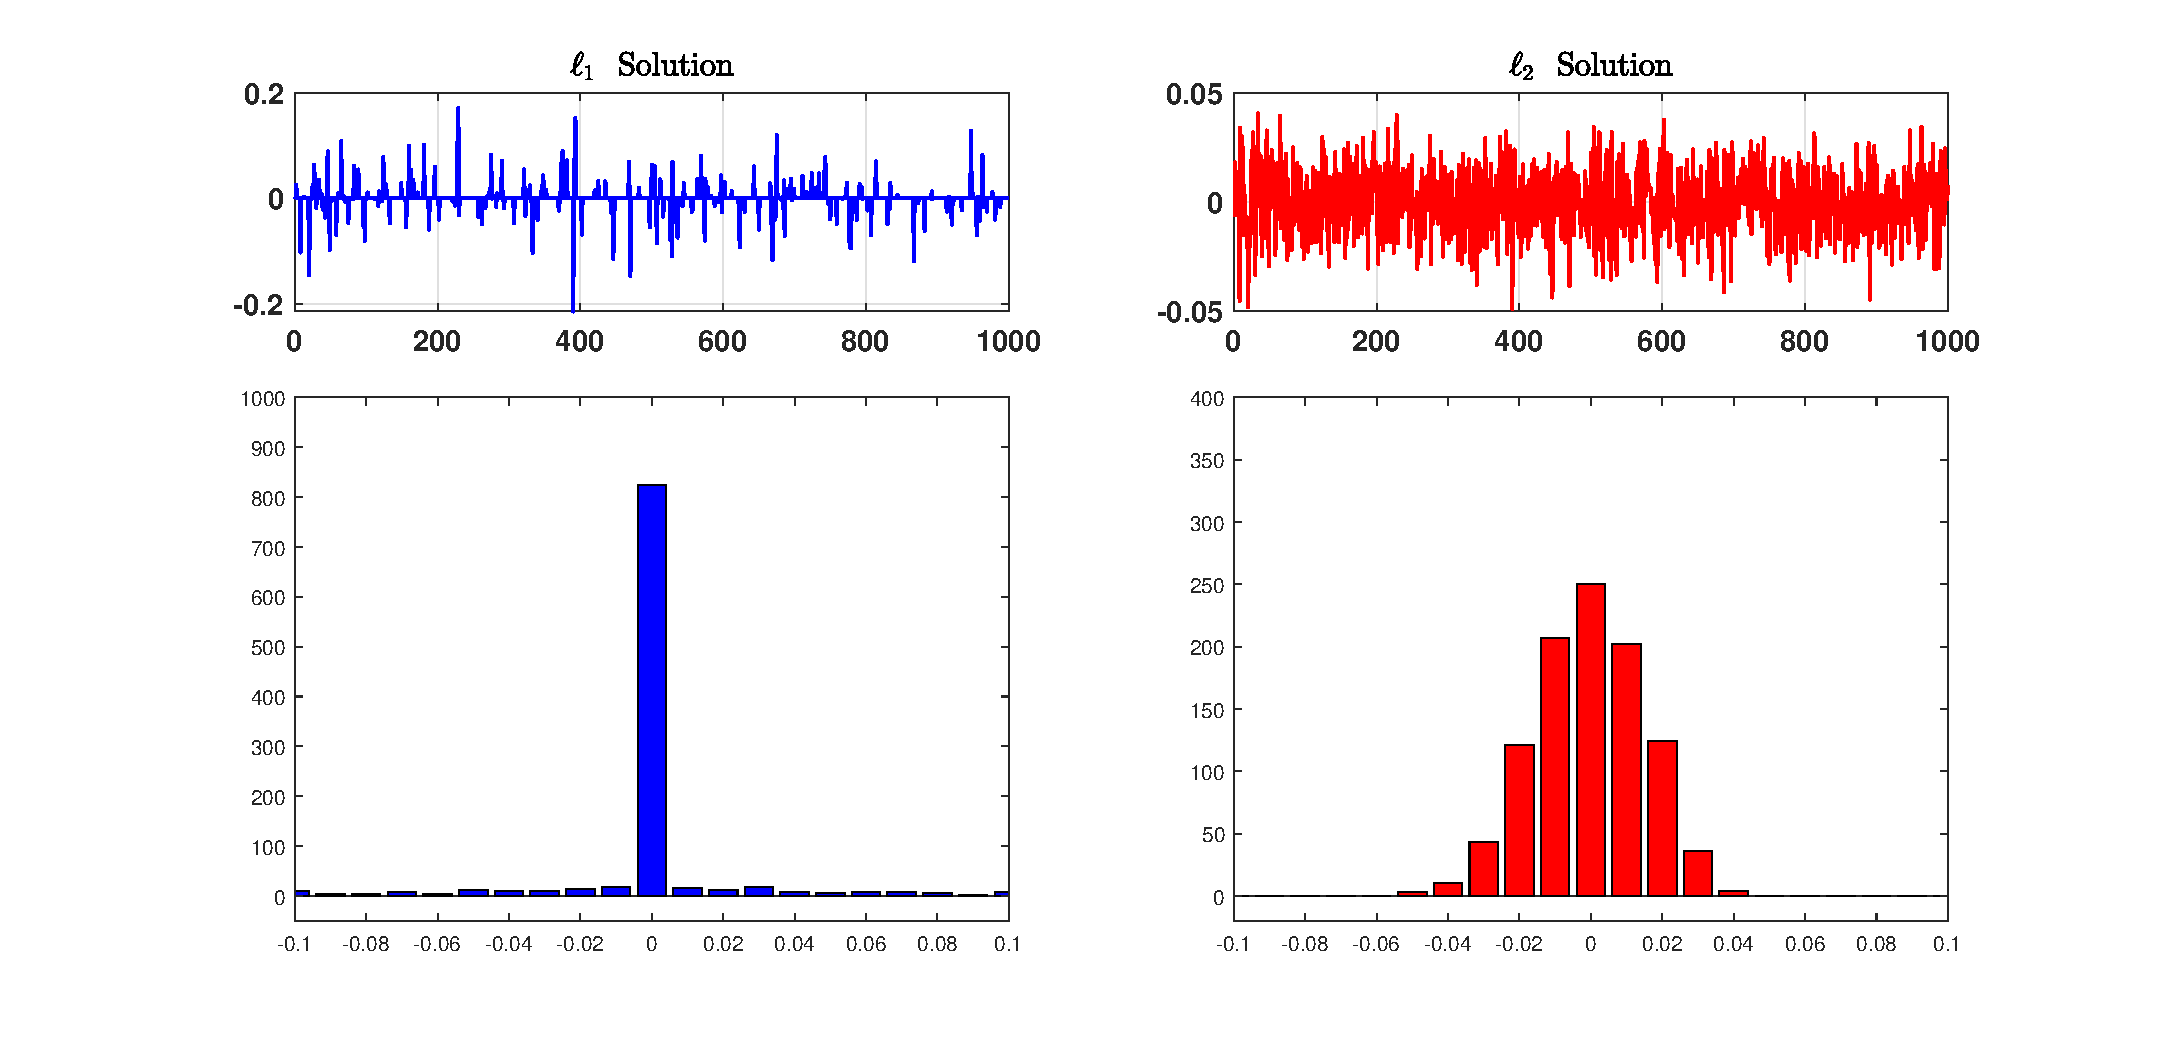
\includegraphics[width = 0.7\textwidth, frame]{Figures/Compressed_Sensing/l1_l2_comparison}
\caption{$\ell_1 ~$ and $\ell_2 ~$ Comparison}
\label{fig:Compressed_Sensing:l1_l2_comparison}
\end{figure}


In $\ell_1 ~$ plot:

\begin{itemize}
    \item Most of the values are 0, and the rest of the elements have some value much greater then 0
    
        
        \begin{itemize}
            \item In fact, by looking at the histogram, we can see that we have 800 value that are 0, and the rest (which are 200 elements since the dimension of the vector $s$ is 1000) are different then 0
        \end{itemize}    
    
    
\end{itemize}

In $\ell_2 ~$ plot:

\begin{itemize}
    \item Most of the elements have some values tends to 0, so no sparse solution as in $\ell_1 ~$ method
\end{itemize}

\subsection{Working with Cos Signals}

\todo{Cos Example}

This is the example of reconstructing cos signal from downsampled measurements.\\

To be rewritten later.


\section{Undetermined Linear System}


We consider the linear system $A_{n \, \times \, m} \, \Vec{x}_{m \, \times \, 1} \, = \, \Vec{b}_{n \, \times \, 1}$, where $m \, > \, n \rightarrow$ we have more unknowns then equations.\\

Under the assumption that $A$ is a full rank matrix, we have infinite solution to this linear system, and from engineering perspective, we can't work with possibly infinite solution, this is impractical.

So what can we done to narrow down the solution ?\\

One way to do this is through regularization, where we assign each solution with some grade, and the best solution has the best grade.\\

As a mathematical notation, we can write it as:

\begin{equation}
\min_x J(x) \quad \text{subject to }  A_{n \, \times \, m} \, \Vec{x}_{m \, \times \, 1} \, = \, \Vec{b}_{n \, \times \, 1}    
\end{equation}

$J(x)$ is the regularization term , and in our case, the lower it is the better.\\

In geometric sense, we are searching over all the possible solution which minimize the levels of $J(x)$.


\begin{figure}[h]
\centering
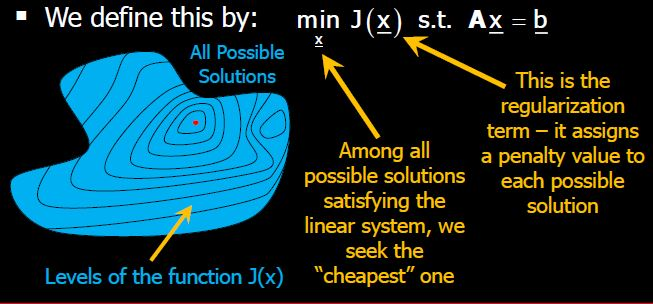
\includegraphics[width = 0.7\textwidth, frame]{Figures/Compressed_Sensing/regularization}
\caption{regularization to narrow down infinite solution to $A \, x \, = \, b$}
\label{fig:Compressed_Sensing:regularization}
\end{figure}

So a natural question to ask: what type of regularization we choose ?\\

For many years, the $\ell_2 ~$ regularizer of the form $J(x) \, = \, \displaystyle\frac{1}{2} \, \lVert B \, x \rVert_2^2$ has been chosen, due to many reasons:

\begin{itemize}
    \item It provide a closed form solution
    
    \item Easy to analyse
    
    \item It presents a unique solution
\end{itemize}

\newpage
The closed form solution of $x$ is shown in \autoref{fig:Compressed_Sensing:closed_form_l2_norm}, where we have derived the gradient of the Lagrangian and null it to obtain a solution of $x$ in function of $\lambda$.\\

Then using $A \,x \, = \, b$, we solve for $\lambda$, and hence obtain a final result of $x$ as a function of the regularizer $B$, the measurements $b$ and $A$.


\begin{figure}[h]
\centering
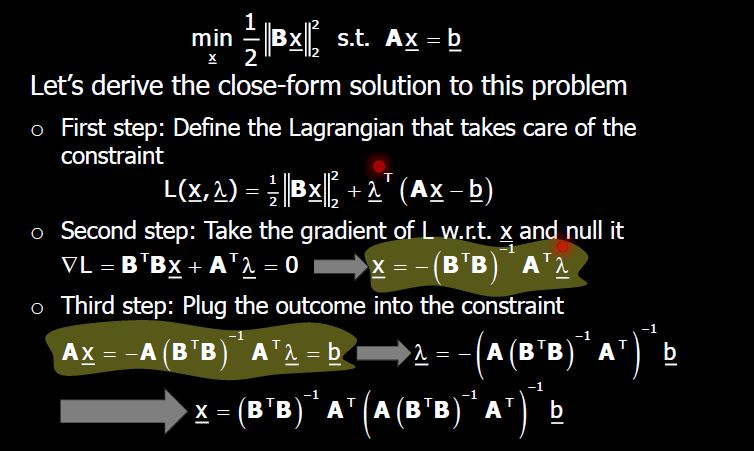
\includegraphics[width = 0.7\textwidth, frame]{Figures/Compressed_Sensing/closed_form_l2_norm}
\caption{Closed form solution of $x$ using $\ell_2 ~$ norm}
\label{fig:Compressed_Sensing:closed_form_l2_norm}
\end{figure}


\subsection{Beyond $\ell_2 ~$ Norm}

The $\ell_2 ~$ norm is not the only norm we can use for the regularizer $J(x)$. Other norms also can be used.\\

$L_p$ norm indeed can be used also because they are convex $\rightarrow$ they provide a unique solution for our problems.\\

\todo{Convexity}: to be rewritten later.

\underline{Idea discussed:}\\

\begin{itemize}
    \item Definition of convexity: convex set, convex function
        
         \begin{itemize}
             \item Many definitions for convexity: using gradient, Hessian, geometry,$\cdots$
         \end{itemize}
    
    \item Difference between strictly convex and convex (to be done later)
    
\end{itemize}

\newpage
\subsection{$\ell_1 ~$}




The interesting norm we will focus on is the $\ell_1 ~$ norm because it promotes sparse solution. 

The initial problem was:

\begin{equation}
\min_x J(x) \quad \text{subject to }  A_{n \, \times \, m} \, \Vec{x}_{m \, \times \, 1} \, = \, \Vec{b}_{n \, \times \, 1}    
\end{equation}

But now we are interested in:

\begin{equation}
\min_x \lVert x \rVert_1 \quad \text{subject to }  A_{n \, \times \, m} \, \Vec{x}_{m \, \times \, 1} \, = \, \Vec{b}_{n \, \times \, 1}    
\end{equation}


In \autoref{fig:Compressed_Sensing:l1_norm_sparse_solution}, we have an example of a linear system of 2 unknowns.

\begin{figure}[h]
\centering
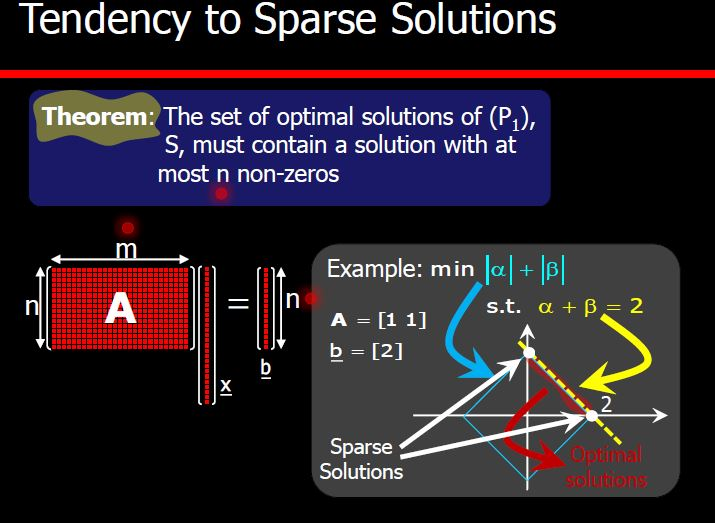
\includegraphics[width = 0.7\textwidth, frame]{Figures/Compressed_Sensing/l1_norm_sparse_solution}
\caption{$\ell_1 ~$ promotes Sparse Solution}
\label{fig:Compressed_Sensing:l1_norm_sparse_solution}
\end{figure}

The optimal solutions is the intersection between the $\ell_1 ~$ plot and the straight line, and the sparse solution is the intersection with the $x$ and the $y$ axis.\\


\todo{Proof and linear programming}

\begin{itemize}
    \item To redo the proof why $\ell_1 ~$ give the sparse solution
    
    
    \item $\ell_1 ~$ problems can be solved using linear programming tools since the structure of the $\ell_1 ~$  problem is similar to linear program $\min_x c^T \, x \, = \, $ subject to $A \, x \, = \, b$ and $x \, > \, 0$
\end{itemize}


%*********************************
%*********************************
%*********************************

\chapter{Two Ortho Case}

\section{Why the 2 ortho case}

Now we begin to study the $P_0$ problem, denoted as:

\begin{equation}
(P_0) \, \,   \min_x \lVert x \rVert_0 \quad \text{subject to }  A_{n \, \times \, m} \, \Vec{x}_{m \, \times \, 1} \, = \, \Vec{b}_{n \, \times \, 1}
\label{Eq:2_Ortho_Case:P0_Problem}
\end{equation}

The $P_0$ problem is very demanding, since any perturbation in $\Vec{b}$ or the matrix $A$ can perturb the solution vector $\Vec{x}$.\\

The goal of studying the $P_0$ problem is due to historical reasons: this is how the sparsity begins, then researchers discovers that this kind of problem is hard to solve and tends toward more intuitive solution.\\


A special case of the $P_0$ problem is the orthogonal case where $A \, = \, [\Psi \, , \, \Phi]$

\begin{figure}[h]
\centering
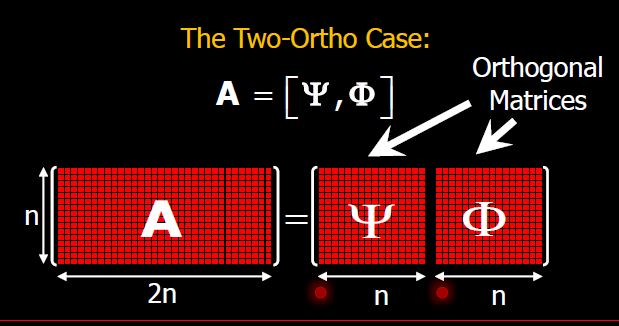
\includegraphics[width = 0.7\textwidth, frame]{Figures/Two_Ortho_Case/Two_Ortho_Definition}
\caption{2 Ortho case Definitions}
\label{fig:Two_Ortho_Case:Two_Ortho_Definition}
\end{figure}


\underline{Recall of the properties for orthogonal matrices:}\\


\begin{itemize}
    \item The transpose is the inverse $\Psi \, \Psi^T \, = \, \Psi^T \, \Psi \, = \, I$
    
    \item The columns (or rows) are orthogonolized to each other and normalized
    
    \item Solution to $\Psi \, \Vec{x} \, = \, \Vec{b}$ is $\Vec{x} \, = \, \Psi^T \, \Vec{b}$
    
    \item Multiplication by these matrices don't change its energy $\rightarrow \lVert \, \Psi \, \Vec{x} \, \rVert_2^2 \, = \, \lVert \,  \Vec{x}  \, \rVert_2^2$
    
    
\end{itemize}

As for the part for the 2 ortho case, it tends to make the solution sparse as shown in the example of \autoref{fig:Two_Ortho_Case:Example_Two_Ortho}. 

\begin{figure}[h]
\centering
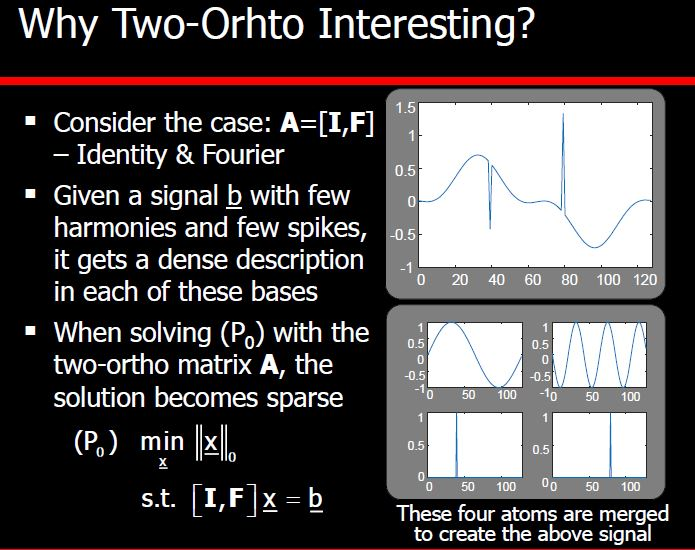
\includegraphics[width = 0.7\textwidth, frame]{Figures/Two_Ortho_Case/Example_Two_Ortho}
\caption{2 Ortho case with $I$ and Fourier Matrix}
\label{fig:Two_Ortho_Case:Example_Two_Ortho}
\end{figure}


A fundamental tool in our analysis for the $P_0$ problem and the 2 ortho case is the \tbi{mutual coherence}, which quantify the similarity between matrices (here $\Psi$ and $\Phi$), defined as the max absolute value between the inner product of the columns between $\Psi$ and $\Phi$:

\begin{equation}
    \mu(\Psi \, , \,\Phi ) \, = \, \max_{1  \leq i \, , \, 1 \leq j} \lvert \Psi_{-,i}^T \, \Phi_{-,i} \rvert
\end{equation}

If $\Psi$ and $\Phi$ have same column, then $\mu(\Psi \, , \,\Phi ) \, = \, 1$, in which we will see later that corresponds to worst case scenario.\\

\newpage
In \autoref{fig:Two_Ortho_Case:All_inner_products}, we have all the possible value for the inner product between $\Psi$ and $\Phi$, which is encapsulated in $\Psi^T \, \Phi$.

\begin{figure}[h]
\centering
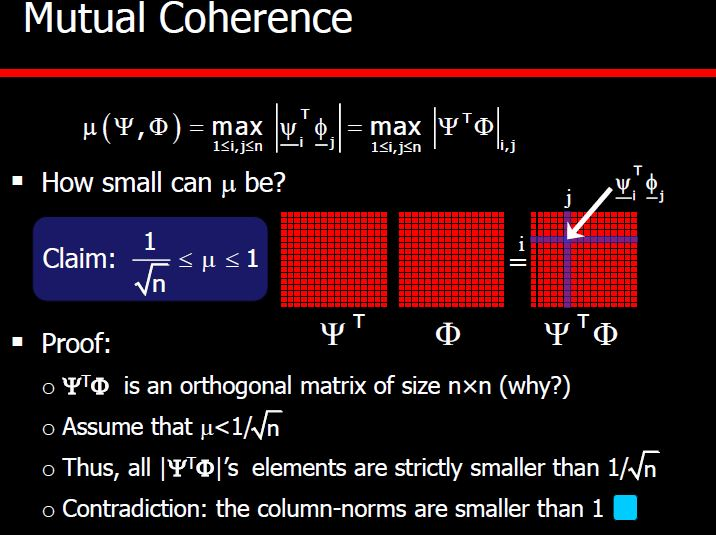
\includegraphics[width = 0.7\textwidth, frame]{Figures/Two_Ortho_Case/All_inner_products}
\caption{All combination of inner product between $\Psi$ and $\Phi$}
\label{fig:Two_Ortho_Case:All_inner_products}
\end{figure}

The $\mu(\Psi \, , \,\Phi )$ is bounded between $\displaystyle\frac{1}{\sqrt{n}}$ and 1.

\section{Uncertainty Principle}

Before keep diving to characterize the uniqueness of the $P_0$ problem, we make a small divergence and introduce the uncertainty theorem in the context of sparse vectors.\\

Given the measurement vector $\Vec{b}$, represented using some vector $\Vec{\alpha}$ and $\Vec{\beta}$ using the relations $\Vec{b} \, = \, \Psi \, \Vec{\alpha}$ and $\Vec{b} \, = \, \Phi \, \Vec{\beta}$, can $\Vec{\alpha}$ and $\Vec{\beta}$ can be jointly sparse?\\

The answer is no, and this is what the uncertainty principle states:


\begin{equation}
    \lVert \Vec{\alpha} \rVert_0 \, + \, \lVert \Vec{\beta} \rVert_0 \geq \, \displaystyle\frac{2}{\mu(\Psi \, , \,\Phi )}
\end{equation}

The sparsity of $\Vec{\alpha}$ and $\Vec{\beta}$ is lower bounded by the threshold $\displaystyle\frac{2}{\mu(\Psi \, , \,\Phi )}$

As a practical implication of this theorem, if we take $[\Psi \, , \, \Phi] \, = \, [I \, , \, F]$, this means that a signal $x$ can't be jointly sparse in the time and the Fourier domain.\\

\todo{Uncertainty}: didn't understand the last example in slide 22 where the picket fence signal is applied to the uncertainty rule.


\section{From Uncertainty to Uniqueness}

\underline{Notes:}\\

\begin{itemize}

    \item This is the $\mathrm{3}^\mathrm{rd}$ video in the playlist
    
    
    \item The big conclusion: for the ortho case, the optimal solution for the $P_0$ problem is the sparse vector which has a non-zero element below $\displaystyle\frac{1}{\mu(\Psi \, , \,\Phi )}$
    
        \begin{itemize}
            \item This conclusion is only for the 2 ortho case
        \end{itemize}
    
    \item This is the proof and theory, the algorithms to fins these solution is to be discussed later.
    
    \item Proof of this theory is to be done later.


\end{itemize}

\section{Spark of a Matrix}

Now we wish to extend the analysis for uniqueness of the 2 ortho case for the matrix $A$ to a more general case, and this is will be done using the spark property.\\

In sections before, we have proceed to divide the matrix $A$ to 2 orthogonals submatrices, but in the general case, this division can't be done, but it will inspire us for the spark property.

\todo{Spark}: to be revisit this section about the division of the 2 matrices

\subsection{Preliminaries about Spark}

\underline{Definition:}\\

The spark of a matrix $A_{n \, \times \, m}$ is the \tbi{smallest} number of linearly dependent columns.\\


\underline{Example:}\\ 

Insert photo slide 38.


\begin{itemize}
    \item This is the I augmented by 1 column to is right
\end{itemize}


What about the rank? the rank is the \tbi{largest} number of columns that are linearly independent.\\


\underline{Notes about the spark:}

\begin{itemize}
    \item The spark is difficult to compute compared to the computation of the rank, which has polynomial complexity
    
    \item The spark $\in \mathbb{N}$, since it counts the number of columns in $A$
    
    \item The spark can't be 1, since there is no single column which is dependent on him self
    
        \begin{itemize}
            \item The only special case where spark = 1, is the 0 column
        \end{itemize}
    
    \item The bound of a spark is:
    
    \begin{equation}
        1 \leq \text{Spark}(A_{n \times \, m}) \leq n \, + \, 1
    \end{equation}
    
    \item Relation to sparsity: assume that we are given a non-trivial solution to the homogeneous linear system $A \, \Vec{x} \, = \, \Vec{0}$
    
    \begin{equation}
        \text{Spark}(A_{n \times \, m}) \, = \, k \rightarrow \, \lVert x \rVert_0 \geq \, k
    \end{equation}
    
    So the sparse of a matrix give the lower bound of non-sparse components in $\Vec{x}$. And as an explanation, $\Vec{x}$ combines the columns of $A$ to form the 0 vector, so at least $k$ columns are needed in such a combination
    
    \item In slide 45: historical flow for the work of spark properties
    
\end{itemize}

\subsection{Extension of Uncertainty and Uniqueness}

Reading: from slide 47 $\rightarrow$ 54.\\

Main points:

\begin{itemize}
    \item The comparison between the lower bound of 2 ortho case and spark case (slide 50)
    
        \begin{itemize}
            \item Here, the uncertainty law is revisited using the spark of the matrix $A$
        \end{itemize}
    
    
    \item If a solution exist to the system $A \Vec{x} \, = \, \Vec{b}$ such that $\lVert x \rVert_0 < \, \displaystyle\frac{\text{Spark}(A)}{2}$, then $\Vec{x}$ is necessarily the sparsest solution
    
        \begin{itemize}
            \item It is the global optimum to the $P_0$ problem.
            
            \item However, this statement doesn't guarantee to give us the best solution, and the computation of this bound is unfeasible since the computation of the spark it self is difficult
        \end{itemize}
    
    
\end{itemize}

\subsection{A more general mutual coherence}

Reading: from slide 56 $\rightarrow$ 63.\\

Due to the difficulty of computing the spark, a more general definition of the mutual coherence can be established, since the mutual coherence is easier to compute.

\begin{itemize}
    \item $\mathrm{1}^\mathrm{st}$ definition:
    
    \begin{equation}
        \mu(A_{n \times m}) \, = \, \max_{1 \leq i \, \neq \, j \, \leq \, m} \displaystyle\frac{\lvert  \Vec{a}_i^T \, \Vec{a}_j \rvert}{\lVert \Vec{a}_i \rVert_2 \, \lVert \Vec{a}_j \rVert_2}
    \end{equation}
    
    So it is the maximal inner product between the normalized columns
    
    \item Also, we can use the fact that $A^T \, A$ contains all the combination of the inner product between the columns of A. Denoting $A^T \, A \, = G$, an alternative definition is:
    
    \begin{equation}
        \mu(A) \, = \, \max_{1 \leq i \, \neq \, j \, \leq \, m} \lvert G \rvert_{i \, , \, j}
    \end{equation}
    
\end{itemize}


\underline{Lemma:}\\

For an arbitrary matrix $A$ we have:


\begin{equation}
    \text{Spark}(A) \geq \, 1 \, + \, \displaystyle\frac{1}{\mu(A)}
\end{equation}


% *************************************
% *************************************
% *************************************


\chapter{Pursuit Algorithm}

\section{Introduction}

In this chapter, we tend the discussion more practical, focusing on the algorithm which solve our $P_0$ problem:


\begin{equation}
(P_0) \, \,   \min_x \lVert x \rVert_0 \quad \text{subject to }  A_{m \, \times \, n} \, \Vec{x}_{n \, \times \, 1} \, = \, \Vec{b}_{m \, \times \, 1}
\label{Eq:2_Ortho_Case:P0_Problem_2}
\end{equation}

where $m \, < \, n$. There are 2 family of algorithm:

\begin{itemize}
    \item The greedy method which focus on the discrete nature of $\Vec{x}$
    
    \item The relaxation family which tend to smooth the $\ell_0 ~$ norm, and use continuous optimization
    
\end{itemize}

The focus of this chapter will be in greedy part.

\section{Core Concept}

There are many greedy algorithm which try to solve the $P_0$ problem, but they all have common methodology when working. This methodology try to find the support of $\Vec{x}$ sequentially, by finding the support of 1 atom first.\\


\begin{enumerate}

\item This is done by sweeping the $m$ columns of $A_{m \, \times \, n}$, and find the best atom (column of $A$ and 1 element of $\Vec{x}$), which matches $A \, \Vec{x} \, = \, \Vec{b}$.

\todo{Img:} Insert picture of the first iteration

\item Given the atom in step 1, we repeat the same process to obtain the $\mathrm{2}^\mathrm{nd}$ support.

\end{enumerate}

The convergence criteria is when $A \Vec{x} \, - \, \Vec{b} \approx  \, \Vec{0} $.\\

By using this algorithm, we reduce the complexity from $m$ choose $k$ to $\mathcal{O}(m)$ tests.

\section{OMP}

We start now by focusing on an algorithm called orthogonal matching pursuit. Some key points of this algorithm are:

\begin{itemize}
    \item It is a greedy algorithm which build the solution in a sequential manner, by adding 1 non-zero term each time to $\Vec{x}$ at a certain index
    
    \item The solution at some iteration $i$ won't neccassarly explain the $P_0$ problem $\leftrightarrow A \Vec{x}_i \neq \Vec{b}$
    
    
    \item That's why we need a residual vector $\Vec{r}_i$ which capture the difference $\leftrightarrow  \, \Vec{r}_i \, = \, A \Vec{x}_i \, - \, \Vec{b}$

\end{itemize}

 shows the steps of the OMP, where it consists from an initialization part and iteration part.\\
 
 The initialization part set the initial guess of the solution to 0 $\Vec{x}_{i \, = \, 0} \, = \, \Vec{0}$, and the residual will be by consequence 0, and the support is an empty set.\\
 
 In the iteration block, we have:
 
 \begin{enumerate}
     
     \item  Given that we have the previous residual $\Vec{r}_{i \, - \, 1}$, we search for the best column of $A$, denoted as $\Vec{a}$, such that when multiplying by some scalar $z$, it give us the minimum difference to the residual in the $\ell_2 ~$  sense.
     
        \begin{itemize}
            \item This step require $m$ test (equal to the number of columns of $A$), and the output will be a collection of $m$ number $E(i)$ where $1 \, \leq \, i \, \leq \, m$
        \end{itemize}
     
     \item We compare among all these $E(i)$ and choose the minimum one.\\
     
     Say that the minimum $E(i)$ is of index $i_0$, so what we obtain is the index $i_0$ which we will be added to the support set $S$
     
     \item Update the support $S_k: S_k \, = \, S_{k \, - \, 1} \, \displaystyle\cup \, \{ i_0\}$
     
     \item We update the value of $\Vec{x}$ by solving a least square problem: 
     
     \begin{equation}
         \Vec{x}_k \, = \, \min_{\Vec{x}_k} \lVert A \, \Vec{x} \, - \, \Vec{b} \rVert_2 \quad \text{s.t } \text{ Supp} \{\Vec{x}\} \, = \,  S_k
     \end{equation}
     
     
     \item Update the residual vector: $\Vec{r}_k \, = \, \Vec{b} \, - \, A \, \Vec{x}_k$
     
     
 \end{enumerate}
 
 
 \todo{Notes OMP}: This is to relistend or re-read later:
 
 \begin{itemize}
     \item Why this method called orthogonal ? because once we found some atom, we never choose it again
 \end{itemize}
 

\section{Variation of the OMP}


OMP is one method to prune the tree of search, and it give us the trade off between complexity and accuracy.\\

\subsection{Least-Square OMP}

The least-square OMP is almost as the same as the OMP, but it is difference by choosing the next atom: the OMP relies on the residual vector, whereas least-square OMP does in another way.\\

What the least-square OMP does is it take each atom in the sensing matrix $\boldsymbol{A}$, compute the error in the $\ell_2 ~$ sense (as shown in \autoref{Eq:Greedy_Method:least_Square_OMP}), then repeat this step for the next atom in $\boldsymbol{A}$, till we scan all the columns, then we take the atom which have the smallest error.


\begin{equation}
         E(i) \, = \, \min_{\Vec{x}} \lVert A \, \Vec{x} \, - \, \Vec{b} \rVert_2 \quad \text{s.t } \text{ Supp} \{\Vec{x}\} \, = \,  S_{k \, - \, 1} \cup \{ i \}
\label{Eq:Greedy_Method:least_Square_OMP}
     \end{equation}

\underline{Note:} $S_{k \, - \, 1} \cup \{ i \}$: at each $i$, we add the previous atom $\Vec{a}_i$ to the selected sensing matrix $ \leftrightarrow \, \,[A_{s_{k \, - \,1}} \, , \, \Vec{a}_i]$.

Using this kind of test to choose the best atom, we don't need to solve for the value of $\Vec{x}$ (that is we don't need step 4 in the OMP algorithm), because in each joined atom, we have already done this step.\\

\subsection{Matching Pursuit}

MP is another variation of OMP, which less complex (so less accurate), but faster then OMP. The difference in MP is the least square update of step 4 in the OMP algorithm.\\

In OMP, when it comes to updating the solution $\Vec{x}_k$, it solve it from scratch using a least square approach, and doesn't rely on the previous solution (coming from previous step).\\

The MP does rely on previous step: what it does it keep the previous solution $\Vec{x}_{k \, - \, 1}$, and add the new atom as shown in \autoref{Eq:Greedy_Method:MP}:

\begin{equation}
    \Vec{x}_k (i_0) \, = \, \Vec{x}_k (i_0) \, + \, \langle  \, \Vec{a}^T_{i_0} \, , \,  \Vec{r}_{k \, - \, 1}  \, \rangle
    \label{Eq:Greedy_Method:MP}
\end{equation}


\subsection{Weak Matching Pursuit}

WMP has its diffference in chosing the next atom.\\

Recall that MP choose the next atom by computing the combination of inner product $\lvert \boldsymbol A \, \Vec{r}_{k \, - \, 1} \rvert$, and then choose the largest entry. For a large matrix, this computation can by huge, and what WMP does in this case for choosing the next atom is by sequential computation (1 step at a time): instead  of computing  $\lvert \boldsymbol A \, \Vec{r}_{k \, - \, 1} \rvert$, it computes $\lvert \langle  \, \Vec{a}^T_{i_0} \, , \,  \Vec{r}_{k \, - \, 1}  \, \rangle \rvert$ and stop when the value obtained is large.\\

How do we know the value is large?

It has been shown that the maximal value of  $\lvert \langle  \, \Vec{a}^T_{i_0} \, , \,  \Vec{r}_{k \, - \, 1}  \, \rangle \rvert$ is upperbouned by the norm of the residual vector $\leftrightarrow \, \lvert \langle  \, \Vec{a}^T_{i_0} \, , \,  \Vec{r}_{k \, - \, 1}  \, \rangle \rvert \, \leq \, \lVert \Vec{r}_{k \, - \, 1} \rVert_2$, so we set some threshold $t$ such that $0 \, < \, t \, < \, 1$, and when the inner product pass the maximum we stop.


For $t \, = \, 1$, the algorithm is slow and do the test for all the atoms (WMP is equivalent to MP in this case), and if $t \, = \, 0$, the algorithm runs fast but it choose a poor quality atom.

\section{Thresholding Algorithm}

\underline{Slides:} 37 $\rightarrow$ 41. \\


Thresholding Algorithm is one of the simplest pursuit algorithm, but it is so popular and has many application.\\

Thresholding algorithm reduce plays on the part of choosing the next atom: what is does is it in the $\mathrm{1}^\mathrm{st}$ step it computes the matrix-vector product $\boldsymbol A^T \, \Vec{b} \, = \, \Vec{\beta}$, then sort the elements of $\Vec{\beta}$ in descending order $i_1 \, , \, i_2 \, \cdots \leftrightarrow \, \lvert \beta_{i_1} \rvert \, \geq \, \lvert \beta_{i_2} \rvert \, \geq \, \lvert \beta_{i_3} \rvert \, \geq \,  \cdots \, \geq \, \lvert \beta_{i_k} \rvert$. This will give the order of atom in which they join the support, and hence we have don't need to repeat in next iterations what atoms do we need to join the support.\\

After this step, threhsolding algorithm act lik OMP: we start by an empty support, we update it and solve the least square problem per step to solve for $\Vec{x}_k$, and the residual is used to stop the algorithm.\\

The burden of choosing the next atom is eased in the thresholding algorithm: in OMP, we need to perform $m \, n \, k$ operations for $k$ atoms, whereas in thresholding we need only $m \, n$ operation only.\\


\todo{Thresholding:} to be done later.

One final note: for a large matrix $\boldsymbol A$, the least square problem to find $\Vec{x}_k$ may be very complex, and instead of solving the least square, we can approximate $\Vec{x}_k$ as: $\Vec{x}_k \, = \, \boldsymbol A_{S_k}^T \, \Vec{b}$ (this should remind us of the MP algorithm)


\newpage
\section{Test Case and Performance Evaluation}

\underline{Slides:} 42 $\rightarrow$ 49.\\

\todo{Test and Performance:} To be relisten very carefully to this video nb 5.\\

The test case consist of drawing some matrix $\boldsymbol A$ and some sparse vector $\vec{x}$, multiplying them so we can obtain our measurement $\vec{y}_{m \,  \times \, 1}$, then feed the measurement and the matrix $\boldsymbol A$ to different solver and compare the estimated solution $\hat{\vec{x}}$ to the true one.\\

Several points need to be considered:

\begin{itemize}
    
    \item $\boldsymbol A$ is of size $50 \, \times \, 200$
    
    \item The sparse vector $\vec{x}$ 
    
        \begin{itemize}
            \item its sparsity is small compared to the dimension of the measurement vector $\vec{y} \leftrightarrow \lVert \vec{x} \rVert_0 \ll m$
            
            \item The non-zero values are random drawn from the interval $[1\, , \, 2]$ or $[-1\, , \, -2]$
            
                \begin{itemize}
                    \item We stay away from $[-1\, , \, 1]$ to avoid values close to 0, which can affect the performance of the algorithm
                \end{itemize}
            
            
        \end{itemize}
    

\end{itemize}

As KPI, we can use the following:

\begin{enumerate}
    \item Relative error:
    
    \begin{equation}
        \text{Error}_{L_2} \, = \, \displaystyle\frac{\lVert  \hat{\vec{x}} \, - \, \vec{x} \rVert_2^2 }{\lVert \vec{x} \rVert_2^2}
    \end{equation}
    
    
\item We can also asses support recovery based on the normalized intersection of the true and the estimated support by applying the following equation:

\begin{equation}
 \text{Error}_{S} \, = \, 1 \, - \, \displaystyle\frac{\lvert \hat{S} \rvert \, \cap \, \lvert S \rvert}{\max \left\{ \lvert \hat{S} \rvert \, , \,  \lvert S \rvert  \right\} }  
\end{equation}
 
If the 2 support don't overlap, their intersection is 0 and hence $\text{Error}_{S}$ is equal to 1
\end{enumerate}

\todo{Analysis}\\


    \begin{itemize}
        \item Relisten to the analysis of the graph in the slide after reprogramming the codes.\\

In evaluation the support metric, the author prune the small values below $10^{-4}$, to avoid counting non-zero element that are effectively zeros (didn't really understand it, to redo it again after simulation)


    \item Advantage and Disadavantages of these test: they are conditioned by low cardinality of $S$ (to be reread from the book later)

    \end{itemize}


\section{Beyond Greedy Relaxation Methods}

Recall the $(P_0)$ problem:


\begin{equation}
(P_0) \, \,   \min_x \lVert x \rVert_0 \quad \text{subject to }  A_{m \, \times \, n} \, \Vec{x}_{n \, \times \, 1} \, = \, \Vec{b}_{m \, \times \, 1}
\label{Eq:2_Ortho_Case:P0_Problem_3}
\end{equation}

where $m \, < \, n$.\\

In sections before, we seen greedy algorithm which tends to approximate the solution of the $P_0$ problem. If we take the $P_0$ problem as optimization problem, there are rich literature in continuous optimization, so we don't use them? this is because the $\ell_0 ~$ is highly non-smooth, and hence we need to relax it to become smooth enough without loosing the essence of sparsity.\\


The $\ell_0 ~$ norm tends to count the number of non-zero element in some vector $\vec{x}$. This can be done using some indicator function $\rho$ as shown in \autoref{fig:Greedy_Methods:Indicator_Function}

\begin{figure}[h]
\centering
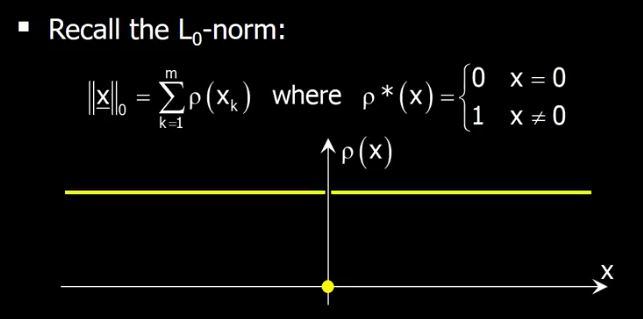
\includegraphics[width = 0.7\textwidth, frame]{Figures/Greedy_Methods/Indicator_Function}
\caption{Indicator function $\rho$ implementing $\ell_0 ~$ norm}
\label{fig:Greedy_Methods:Indicator_Function}
\end{figure}

\newpage
So how can we relax the $\ell_0 ~$ norm? 

Some examples of smoother function are shown in \autoref{fig:Greedy_Methods:smoother_function}

\begin{figure}[h]
\centering
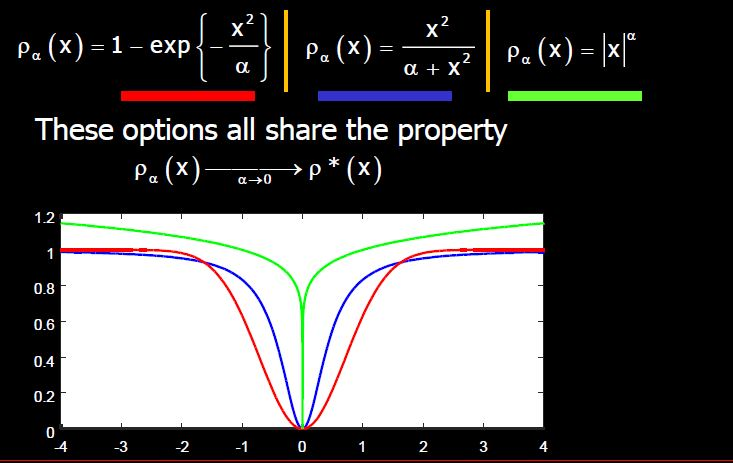
\includegraphics[width = 0.7\textwidth, frame]{Figures/Greedy_Methods/smoother_function}
\caption{Example of some smoother function}
\label{fig:Greedy_Methods:smoother_function}
\end{figure}

The common things about all these function, is that as $\alpha \rightarrow \, 0$, the smoother function behaves exactly as the original $\ell_0 ~$ norm.\\

Another tool used combined with smoother function is what we called graduate optimization, shown in \autoref{fig:Greedy_Methods:graduate_optimization}:

\begin{figure}[h]
\centering
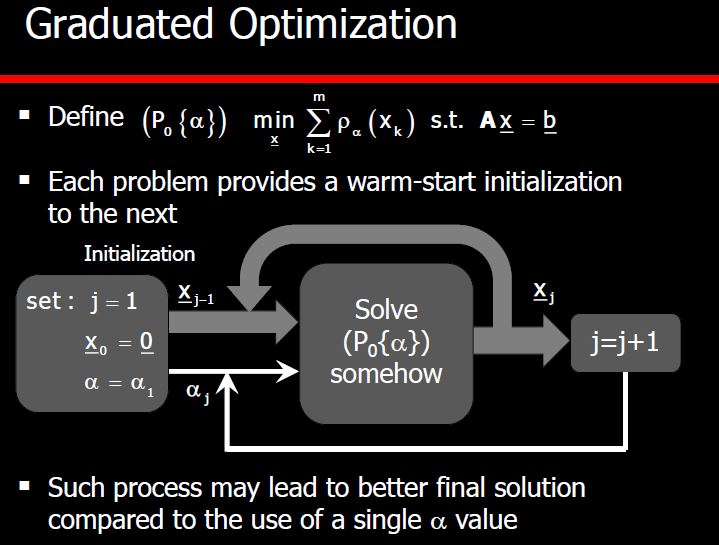
\includegraphics[width = 0.7\textwidth, frame]{Figures/Greedy_Methods/graduate_optimization}
\caption{Graduate Optimization}
\label{fig:Greedy_Methods:graduate_optimization}
\end{figure}

\begin{itemize}
    \item We use the smoothed version of the $P_0$ problem
    
    \item We initialize the algorithm with some high value of $\alpha$, then decrease it
    
    \item The trick in this algorithm is that we use the previous solution $\vec{x}_{j \, - \, 1}$ as initial guess in the next iteration: this trick is named warm start, and avoid us many local minima
\end{itemize}

An instance of the class of the graduate optimization is what is called the IRLS (iterative reweigthed least square), in which we solve the smooth version of the $P_0$ by rewriting the smoothed indicator function $\rho_{\alpha}(x)$ as $\displaystyle\frac{\rho_{\alpha}(x)}{x_k^2} \, \times \, x_k^2$, and hence the term $ \displaystyle\frac{\rho_{\alpha}(x)}{x_k^2}$ is considered as some fixed weights $w_k$, in which we will update it in the algorithm.\\

The last relaxation method is $\ell_1 ~$ norm, which is a convex relaxation since the $\ell_1 ~$ is convex. The $\ell_1 ~$ norm relaxation is known as basis pursuit.

%***************************************
%***************************************
%***************************************

\chapter{From Exact to Approximate Solution}

\section{Preliminary}

In previous chapter, we have seen many algorithm to solve the $(P_0)$ problem: started from greedy algorithm, then for some relaxation method (such as FOCCUS and Basis pursuit). However, there is some slight problem in the formulation of the $(P_0)$ problem. Recall its structure:

\begin{equation}
(P_0) \, \,   \min_x \lVert \vec{x} \rVert_0 \quad \text{subject to }  \boldsymbol A_{m \, \times \, n} \, \Vec{x}_{n \, \times \, 1} \, = \, \Vec{b}_{m \, \times \, 1}
\label{Eq:2_Ortho_Case:P0_Problem_4}
\end{equation}

where $m \, < \, n$.\\

The equality constraints in \autoref{Eq:2_Ortho_Case:P0_Problem_4} is too strict: in reality, we don't obtain exactly the measurement vector $\Vec{b}_{m \, \times \, 1}$ in such clean way, it is usually contaminated by noise, so we need to reformulate the $(P_0)$ problem into a more adaptive version, which handle the noise in  $\Vec{b}_{m \, \times \, 1}$. This reformulation will be called $(P_0^{\epsilon})$ shown in \autoref{Eq:2_Ortho_Case:P0_Problem_4}:


\begin{equation}
(P_0^{\epsilon}) \, \,   \min_x \lVert \vec{x} \rVert_0 \quad \text{subject to }  \lVert \,  \boldsymbol A_{m \, \times \, n} \, \Vec{x}_{n \, \times \, 1} \, - \, \Vec{b}_{m \, \times \, 1} \, \rVert_2^2 \leq \epsilon^2
\label{Eq:2_Ortho_Case:P0_Problem_4}
\end{equation}


\todo{Reformulating P0}\\

\begin{itemize}
    \item Why we add noise to $\vec{x}$: in what engineering scenarios do we have such case ?
\end{itemize}

In this chapter, we shall see pursuit algorithm and conditions to solve $(P_0^{\epsilon})$


\section{Greedy Algorithm}

The greedy algorithm (OMP, MP, $\cdots$) all tends to conserve their properties when solving the $(P_0^{\epsilon})$ problem (like for OMP: never choose an the same atom twice).

These algorithm will have the same step, the only thing we need to modify is to add the $\epsilon$ we use in \autoref{Eq:2_Ortho_Case:P0_Problem_4} when testing for the convergence of the residual.\\

\newpage
\section{Basis Pursuit}

As for the basis pursuit algorithm which uses the $\ell_1 ~$ 

\begin{equation}
(P_1^{\epsilon}) \, \,   \min_x \lVert \vec{x} \rVert_1 \quad \text{subject to }  \lVert \, \boldsymbol A_{m \, \times \, n} \, \Vec{x}_{n \, \times \, 1} \, - \, \Vec{b}_{m \, \times \, 1} \, \rVert_2^2 \leq \epsilon^2
\label{Eq:Exact_to_approx:P1_Problem_noisy}
\end{equation}

\autoref{Eq:Exact_to_approx:P1_Problem_noisy} can't be solved using linear programming to: it involves more advanced programming called quadratic programming.


\subsection{IRLS for Noisy Basis Pursuit}

In this part, we revisit the IRLS algorithm to use it in order to solve the $P_1^{\epsilon}$ problem. 

Instead of handling \autoref{Eq:Exact_to_approx:P1_Problem_noisy} directly in its constraint form, we will replace it by an equivalent form know as the Lagrangian, which uses a penalty term $\lambda$ instead of the constraint $\epsilon$ in \autoref{Eq:Exact_to_approx:P1_Problem_noisy}. The follwing formulation is as follows:

\begin{equation}
\hat{\vec{x}} \, = \, \argmin_{\vec{x}} \lambda \, \lVert \,  \vec{x} \, \rVert_1 \, + \, \displaystyle\frac{1}{2} \, \lVert \, \boldsymbol A \, \vec{x} \, - \, \vec{b} \, \rVert_2^2 
\label{Eq:Exact_to_approx:P1_Problem_noisy_lagrangian}
\end{equation}

The main idea of the IRLS is to express the $\ell_1 ~$  into and $\ell_2 ~$  form as shown in :


\begin{equation}
\begin{array}{lcl}
\lVert \vec{x} \rVert_1 \, &=& \, \displaystyle\sum_{i \, = \, 1}^m \,  \lvert x_i \rvert \\ \\
                 &=& \, \displaystyle\frac{1}{2} \displaystyle\sum_{i \, = \, 1}^m \left\{ 2\, \lvert x_i \rvert^{-1} \right\} \, \lvert x_i \rvert^2 \\ \\
                 &=& \, \displaystyle\frac{1}{2} \vec{x}^T \, \boldsymbol W (\vec{x}) \, \vec{x} 
\end{array}
\label{Eq:Exact_to_approx:IRLS_l1}
\end{equation}

Plugin in the result of \autoref{Eq:Exact_to_approx:IRLS_l1} in \autoref{Eq:Exact_to_approx:P1_Problem_noisy_lagrangian} we get:

\begin{equation}
 \hat{\vec{x}} \, = \, \argmin_{\vec{x}} \displaystyle\frac{\lambda}{2} \, \vec{x}^T \, \boldsymbol W (\vec{x}) \, \vec{x} \, + \,  \displaystyle\frac{1}{2} \, \lVert \, \boldsymbol A \, \vec{x} \, - \, \vec{b} \, \rVert_2^2
 \label{Eq:Exact_to_approx:IRLS_l1_second_form}
\end{equation}

\autoref{Eq:Exact_to_approx:IRLS_l1_second_form} has a closed form solution by taking its derivative with respect to $\vec{x}$, yielding to the following solution:

\begin{equation}
  \hat{\vec{x}} \, = \, \left[ \, \lambda \boldsymbol W \, + \, \boldsymbol A^T \,  \boldsymbol A \,     \right]^{-1} \, \boldsymbol A^T \, \vec{b}       
\end{equation}


\newpage
Steps of the algorithm is shown in \autoref{fig:Exatct_Approx:irls_l1_noisy}

\begin{figure}[h]
\centering
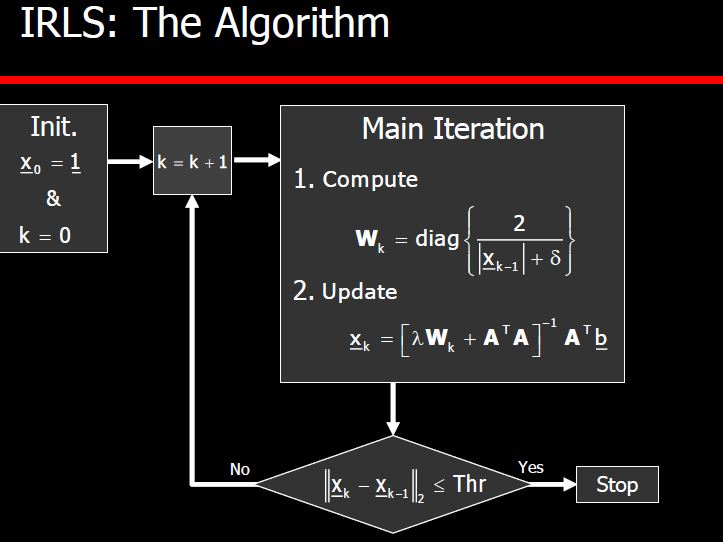
\includegraphics[width = 0.7\textwidth, frame]{Figures/Exatct_Approx/irls_l1_noisy}
\caption{Example of some smoother function}
\label{fig:Exatct_Approx:irls_l1_noisy}
\end{figure}

\todo{IRLS for l1 noisy}

\begin{itemize}
    \item Why we initialize the $\vec{x}$ by 1 instead of 0
    
    \item The convergence of this algorithm 
    
\end{itemize}

%**************** References ****************

\bibliographystyle{IEEEtran}

\bibliography{Literature/Books_Signal_Processing,Literature/Papers_Sampling}


\end{document}










